\documentclass[10pt]{article}
% File icdp2009.sty
% Preamble that you have to include to use the template  

% July 24, 2009
% Contact: simonnet@ecole.ensicaen.fr

\usepackage[a4paper, textwidth=18cm, textheight=24cm, top=1.5cm, bottom=2.85cm, left=1.5cm, right=1.5cm]{geometry}

\usepackage{template/icdp2009}

% left justified caption
\makeatletter
\long\def\@makecaption#1#2{%
\vskip\abovecaptionskip
\sbox\@tempboxa{#1. #2}%
\ifdim \wd\@tempboxa >\hsize
#1. #2\par
\else
\global \@minipagefalse
\hb@xt@\hsize{\box\@tempboxa\hfil}%
\fi
\vskip\belowcaptionskip}
\makeatother




%other package
\usepackage{lmodern}
\usepackage{graphicx}
\usepackage{times}
\usepackage{enumitem}

\begin{document}
\noindent

\bibliographystyle{plain}

\title{Space-time volumes for classification of platform diving tricks}

\authorname{C. Lenzenweger, B. Sespede}

\maketitle

\section{Topic and data}

In this KU we will implement a neural network capable of classifying video recordings of different styles of platform diving. In platform diving the performances are composed by three main stages: takeoff, flight, and entry. The flight stage is the one where the diver is in air and can be sub-classified into the three distinct types shown in Figure \ref{fig:dive-styles} (and a fourth "free" style composed by a combination of the other three). During the jump the performer is expected to do somersaults using these positions. Furthermore, the diver might perform twists when switching between styles in a single dive.

\begin{figure}[!htb]
\center{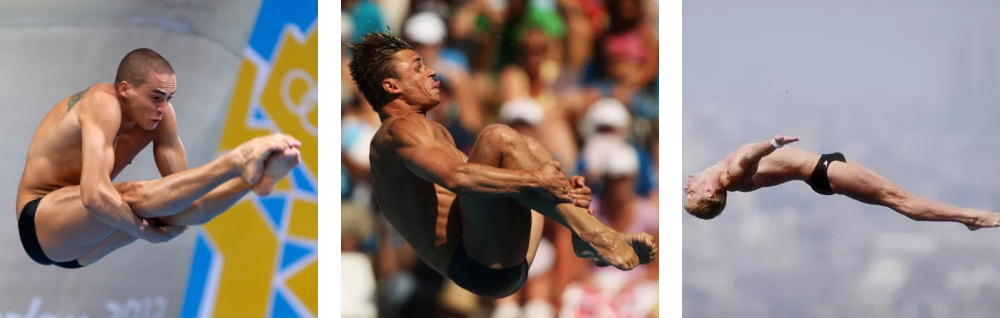
\includegraphics[scale=0.98]
{figures/dives.png}}
\caption{\label{fig:dive-styles} The figure shows the three main flight styles from left to right: pike, tuck, and straight.}
\end{figure}

Our goal is to use space-time volumes (STVs) to extract features that will then be used to train a neural network. This network will then be used to classify the three different flight styles (in previously unseen videos (styles shown in Figure~\ref{fig:dive-styles}). Special importance will be placed in aggregating temporal data to solve possible short-term conflicts during the classification process, as the \emph{pike} and \emph{tuck} position can be easily miss-labeled when seen in certain angles. To train our network we plan to use the \textit{Diving48} dataset \cite{ref-diving48} which contains a large number of recordings from a variety of angles. All the videos in this dataset contain ground-truth labels that describe the sequence in four ways: (i) takeoff type, (ii) the number of somersaults, (iii) the number of twists, and (iv) the flight style.

To simplify the extent of our work we have decided to make certain restrictions to the original dataset. First, we will remove the "free" flight style from the dataset (i.e. the style where the performer combines several styles in one dive). Furthermore, we will clip the recordings to remove the parts where the performer sinks below the water, as the STVs break when doing so. As a last pre-processing step, we will remove the performances with extreme camera angles and twists in them. The intention behind these modifications is to allow us to focus exclusively on flight style classification while keeping it challenging enough.

\section{Envisioned solution}

In order to solve this problem we propose the following pipeline using \emph{OpenCV} and \emph{TensorFlow}:\\

\textbf{Extraction of Space-Time Volumes and Pre-processing.} This step is performed by Filip Ilic and he will provide us with three-dimensional tensors containing the STVs, and other relevant data such as bounding boxes containing the divers and optical flow estimation.

Considering the algorithm for STV extraction can produce small unrelated artefacts, we decided to perform simple morphological operations to improve the accuracy of upcoming feature extractions. Nevertheless, most of these artefacts are outside of the bounding boxes. Only the STVs within the bounding box are taken into account for further processing.\\

\textbf{Feature Extraction and Token Selection.} The token list should represent the pose of the diver completely. To this end, the intended token selection can be roughly divided into four sequential steps:
\begin{enumerate}[nosep]
\item Selection of 2-3 largest STVs in the volume, as they usually represent the skin of the diver.
\item Contour extraction from the selected STVs.
\item Fitting of 2D primitives onto the selected STVs. One of the following primitives will be chosen during development according to performance and quality of end-results: Minimum bounding rectangle (MBR), ellipses, or lines.
\item Extraction of scalar features based on the fitted primitives. The actual set of features finally used, might be reduced based on principal component analysis: (i) Absolute orientation angle, (ii) relative area with respect to bounding box, (iii) distance to the center of the bounding box, (iv) mutual relative orientation angle, (v) mutual relative distance, (vi) elongation or aspect ratio, and (vii) compactness.
\end{enumerate}
\vspace{1em}
\hspace{\parindent}\textbf{Pre-processing in Feature Space.} Any angle in the token list is taken modulo $\pi$ and split up into it's sine and cosine to ensure that similar orientation has similar feature values. The modulo operation represents that the fitted primitive 2D shape is symmetric (i.e. has no ``head'' and ``tail''). Moreover, the sine is multiplied by factor 2 and shifted by -1 to ensure the same range $[-1;1]$.

The area and distance features are scaled to the range $[-1;1]$ with respect to the bounding box of the current frame. A filter will be used to avoid detrimental effects resulting from flickering of the bounding box that might induce rapid unrepresentative changes over time.\\

\textbf{Classification.} The actual classification task will be performed by training a neural network. We intend to compare three different network structures: (i) A convolutional neural network that consists of one-dimensional convolutions, separately for each scalar feature. Additionally, there will be moderate pooling layers. (ii) a neural network with feature vector as input, plus the relative time as scalar in the range [0;1], and (iii) a neural network where the state vector is provided as two-dimensional input. The cross entropy is taken as cost function for each kind of network.

\section{Expected results}

We expect to evaluate how adequate the STVs are for the intended feature set. Moreover, we would like to see if the chosen tokens are suitable for action recognition in the context of platform diving. Finally, we have identified the following difficulties, which we partially address with the proposed solution: (i) how to properly select the most meaningful STVs, and (ii) how to handle inaccurate or temporally inconsistent STVs.

\bibliography{references/references.bib}

\end{document}